\documentclass[12pt,oneside]{book}
\usepackage{geometry}                		% See geometry.pdf to learn the layout options. There are lots.
\geometry{a4paper}                   			% ... or a4paper or a5paper or ... 
%\geometry{landscape}                		% Activate for for rotated page geometry
%\usepackage[parfill]{parskip}    		% Activate to begin paragraphs with an empty line rather than an indent
\usepackage{graphicx}				% Use pdf, png, jpg, or epsß with pdflatex; use eps in DVI mode
								% TeX will automatically convert eps --> pdf in pdflatex		
\usepackage{amssymb}

\usepackage[spanish]{babel}			% Permite que partes automáticas del documento aparezcan en castellano.
\usepackage[utf8]{inputenc}			% Permite escribir tildes y otros caracteres directamente en el .tex
\usepackage[T1]{fontenc}				% Asegura que el documento resultante use caracteres de una fuente apropiada.

\usepackage{hyperref}				% Permite poner urls y links dentro del documento

\title{Mi Juego Favorito}
\author{Javier Tibau}
%\date{}							% Activate to display a given date or no date

\begin{document}
\maketitle
\tableofcontents

\chapter{Introducción}
El libro a continuación es creado como una herramienta para el desarrollo de habilidades de edición colaborativa de documentos de texto plano. La herramienta que habilita dicha colaboración, en este taller, es Git pero podría ser reemplazada por otros sistemas de versionamiento.

\chapter{Los Juegos}

\section{Buscaminas}

\begin{figure}[htbp]
\begin{center}
\includegraphics[width=.60\textwidth]{./imagenes/minesweeper.png}
\caption{Buscaminas}
\label{Buscaminas}
\end{center}
\end{figure}
Buscaminas\footnote{\url{http://minesweeperonline.com/}} es uno de los juegos más jugados debido a lo ubicuo de su distribución. Fue incluido en 1992 en la versión de Windows 3.1 y desde entonces lo hemos encontrado presente en todas las versiones de dicho sistema operativo.
En la figura \ref{Buscaminas} puede ver una implementación web del juego.
La premisa del juego es simple: Limpiar el campo de juego sin hacer explotar ninguna de las minas que se encuentran en la cuadrícula.

\subsubsection{¿Por qué es uno de mis juegos favoritos?}
\begin{itemize}
\item[Javier Tibau] Las reglas del juego son sencillas y fáciles de entender. A pesar de esto, el juego no es atractivo para todo el mundo, creo que es un gusto adquirido. Las reglas me fueron presentadas por mi papá, quien en su máquina de trabajo con Windows 3.11 era uno de los pocos juegos ``divertidos'' que tenía. Para mi, el gran interés del juego es que destaca (o esconde) la resolución de problemas con fondo algebraico. En cierto momento del juego, y para el jugador que ha estudiado álgebra lineal, el reventar una casilla se torna similar a descifrar un sistema de ecuaciones con varias incógnitas. Los sistemas sencillos son bien definidos y tienen 2, 3 o hasta 4 incógnitas, mientras los más complejos pueden inclusive tener múltiples soluciones.
\end{itemize}

\section{Dota 2}

\begin{figure}[htbp]
\begin{center}
\includegraphics[width=.60\textwidth]{./imagenes/dota2.jpg}
\caption{Dota 2}
\label{Dota 2}
\end{center}
\end{figure}
Dota 2 \footnote{\url{http://dota2.com/}} es un juego creado por Valve basado en el popular mod de Warcraft 3, Defense of the Ancients. Es un juego de estrategia en equipo para ser jugado con equipos de 5 personas cada uno.
Dota 2 combina elementos de estrategia en tiempo real con perspectiva "en tercera persona", incorporando a todo ello un sistema de nivelación y jugabilidad de diversos juegos de rol como Diablo. Los jugadores asumen el papel de una unidad clasificado como un "héroe", que puede subir de nivel hasta un máximo de 25. La configuración básica de Dota 2 consiste en dos ciudades de distinta forma, cada una cuenta con una fortaleza de defensa conocida como "ancestro", situadas en los extremos opuestos de un mapa equilibrado de manera uniforme. Entre ellas hay varias regiones de conexión identificado como "caminos", que son atravesados por unidades enemigas, al tiempo que luchan contra poderosas torres defensivas a lo largo del camino. Los jugadores se dividen entre dos equipos, cada uno con hasta cinco jugadores, para competir como los principales defensores de cada Fortaleza de los Ancestros.

\subsubsection{¿Por qué es uno de mis juegos favoritos?}
\begin{itemize}
\item[Victor Cedeño] Este es un juego que requiere de comunicación y cooperación entre 5 personas para poder lograr el objetivo de vencer al otro equipo. Es muy dificil jugar solo sin la ayuda de tus compañeros. El juego tiene una gran selección de más de 100 heroes para elegir, esto quiere decir que cada partida es diferente ya que las combinaciones posibles de los equipos son innumerables. Es un juego que fomenta el trabajo en equipo y las decisiones correctas.
\end{itemize}

\include{juegos/Zelda}
\section{Corazones}

\begin{figure}[htbp]
\begin{center}
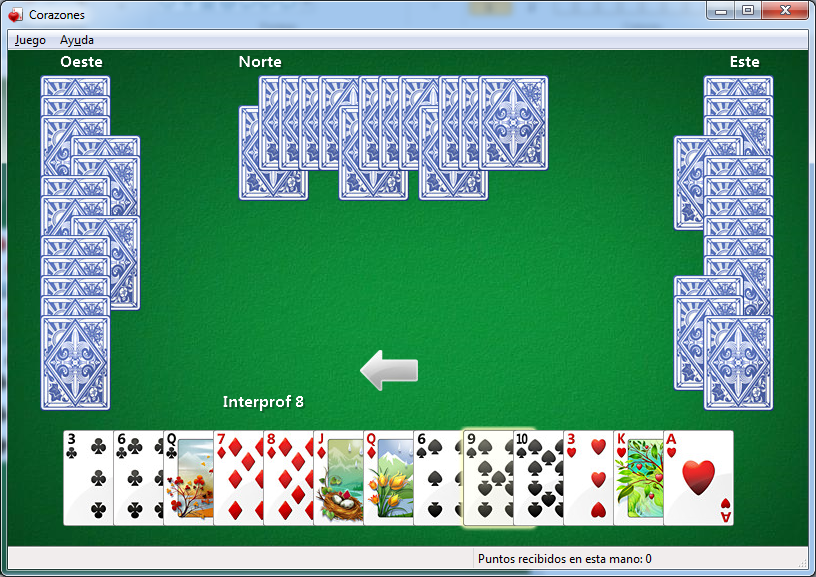
\includegraphics[width=.60\textwidth]{./imagenes/Corazones.png}
\caption{Corazones}
\label{Corazones}
\end{center}
\end{figure}
Corazones\footnote{\url{http://www.magnojuegos.com/juegosonline/corazones/}} es un juego de cartas cuyo objetivo es acabar la partida con el mínimo de puntos posibles. Es una evolución del original "Dama de Picas" francés. El juego estándar se realiza con una baraja francesa y cuatro jugadores. Se ha popularizado mucho a partir de su inclusión en el sistema operativo Windows.
En la figura \ref{Corazones} puede ver una implementación del juego.
La premisa del juego es simple: Tener la menor cantidad de puntos al final de las partidas.

\subsubsection{¿Por qué es uno de mis juegos favoritos?}
\begin{itemize}
\item[Veronica Pozo] Porque es uno de los primeros juegos que venían instalados en Windows y crecí jugando este juego. Es un juego sencillo y facil de entender para cualquier edad. Era muy útil cuando te aburrías de Buscaminas y Carta Blanca. Crecer sin internet nos llevó a aprovechar los juegos que teníamos a la mano. Los juegos de cartas como Solitario, Carta Blanca y Corazones fueron parte de nuestra infancia y a pesar de los nuevos juegos como Solitario Spider creo que los clásicos, con los que crecimos, siempre tendrán unos minutitos de nuestro tiempo.
\end{itemize}

\section{Rayman}

\begin{figure}[htbp]
\begin{center}
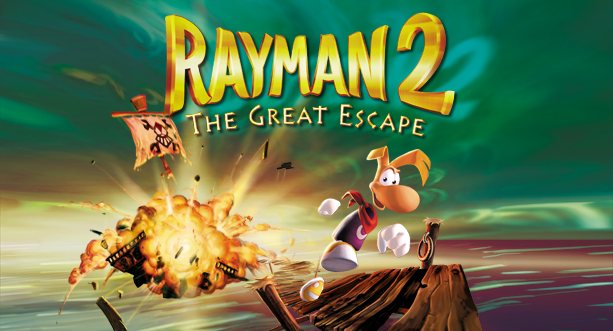
\includegraphics[width=.60\textwidth]{./imagenes/rayman.jpg}
\caption{Rayman}
\label{Rayman}
\end{center}
\end{figure}
Rayman\footnote{\url{http://www.onlinemania.org/juego/11605/Rayman-2--The-Great-Escape-8PSX9.html}} es un juego de aventura donde eres un personaje que debe salvar al mundo de unos malvados piratas roboticos venidos del espacio en naves espaciales con forma de barcos de guerra  gigantescos han invadido el planeta y, capturado y encerrado a la mayoria de sus habitantes. 
Rayman es apresado pero luego logra escapar para buscar Las Cuatro Máscaras, liberando a todo sus amigos, recogiendo los lums de energia y derrotar a los piratas. 
En la figura \ref{Rayman} puede ver una implementación del juego.
La premisa del juego: Recoger los lums de energia y las Cuatro Máscaras.

\subsubsection{¿Por qué es uno de mis juegos favoritos?}
\begin{itemize}
\item[Manuel Suárez] El juego que se me hizo mas fácil jugar, ademas Rayman es un personaje amigable y muy interesante. 
Se basa en un mundo mitico donde los seres son de diferentes razas pero que se apoyan para lograr tener o establecer un estado de paz entre las naciones
este se ve alterado por enemigos que buscan distorsionar este estado y lograr cometer barbaridades. 


\end{itemize}

\section{Fallout3}

\begin{figure}[htbp]
\begin{center}
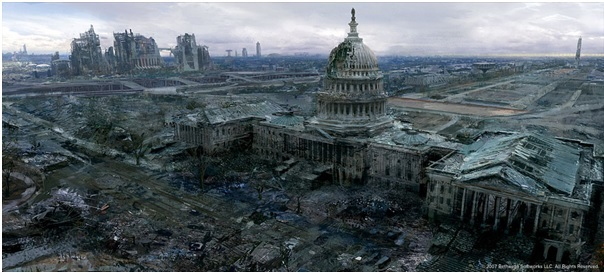
\includegraphics[width=.40\textwidth]{./imagenes/fallout3.jpg}
\caption{Fallout3}
\label{Fallout3}
\end{center}
\end{figure}
Fallout 3 tiene lugar en el año 2278, 200 años después de que una guerra mundial culminara en un holocausto nuclear. La ambientación consiste en una región post-apocalíptica y retrofuturista que abarca gran parte de Washington D.C., e  incluye edificios de la vida real devastados por la guerra como la Casa Blanca y el Monumento a Jefferson. El juego comienza dentro del Refugio 101, donde sus habitantes creen haber nacido originalmente, antes de aventurarse a las afueras del refugio donde se enfrentarán a la peligrosa verdad, un mundo devastado por la guerra, poblado por criaturas mutantes debido a los altos niveles de radiación.  

\subsubsection{¿Por qué es uno de mis juegos favoritos?}
\begin{itemize}
\item[José Salas] En Fallout 3, encarnamos a un niño que vive con su padre y el resto de una comunidad en un bunker, el Refugio 101. Totalmente aislados de los acontecimientos que se suceden en el exterior, y bajo una suerte de civilización con sus propias normas y leyes; la mayoría de sus ciudadanos han crecido ajenos a que en el exterior la tierra ha sido devastada por una guerra nuclear. El principal atractivo de Fallout 3 es el hecho de descubrirlo por nosotros mismos. Eventualmente salimos del refugio y vamos descubriendo este amplio mundo con total libertad.

\end{itemize}

\chapter{Conclusiones}
Cuales juegos fueron más populares y un breve razonamiento del porqué.

\end{document}  
